Make a histogram of the intensity values in your image. Does your image use the entire range of values from 0 to 255? What is the minimum pixel value used? What is the maximum?

\begin{solution}\ 
    \begin{lstlisting}[language=Matlab]
    histogram(X_col)
    \end{lstlisting}

    \begin{center}
        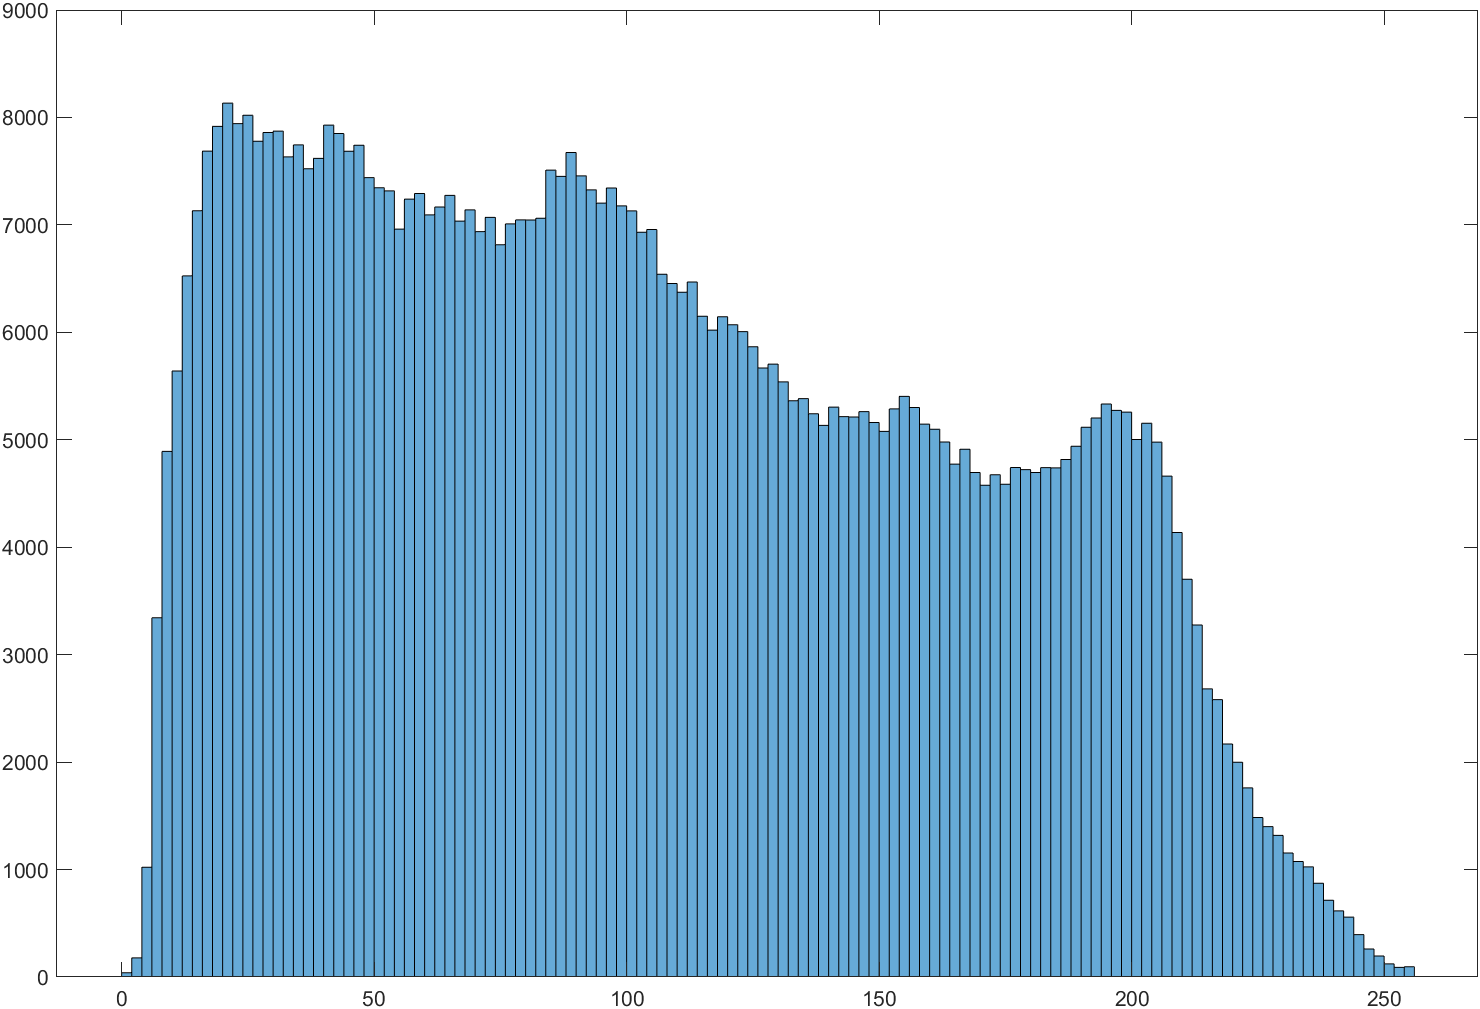
\includegraphics[width=0.8\textwidth]{img/e7p4.png}
    \end{center}
    
    Fortunately, it looks like the image is well-centered and distributed.
\end{solution}